\begin{figure*}[t!]
\centering
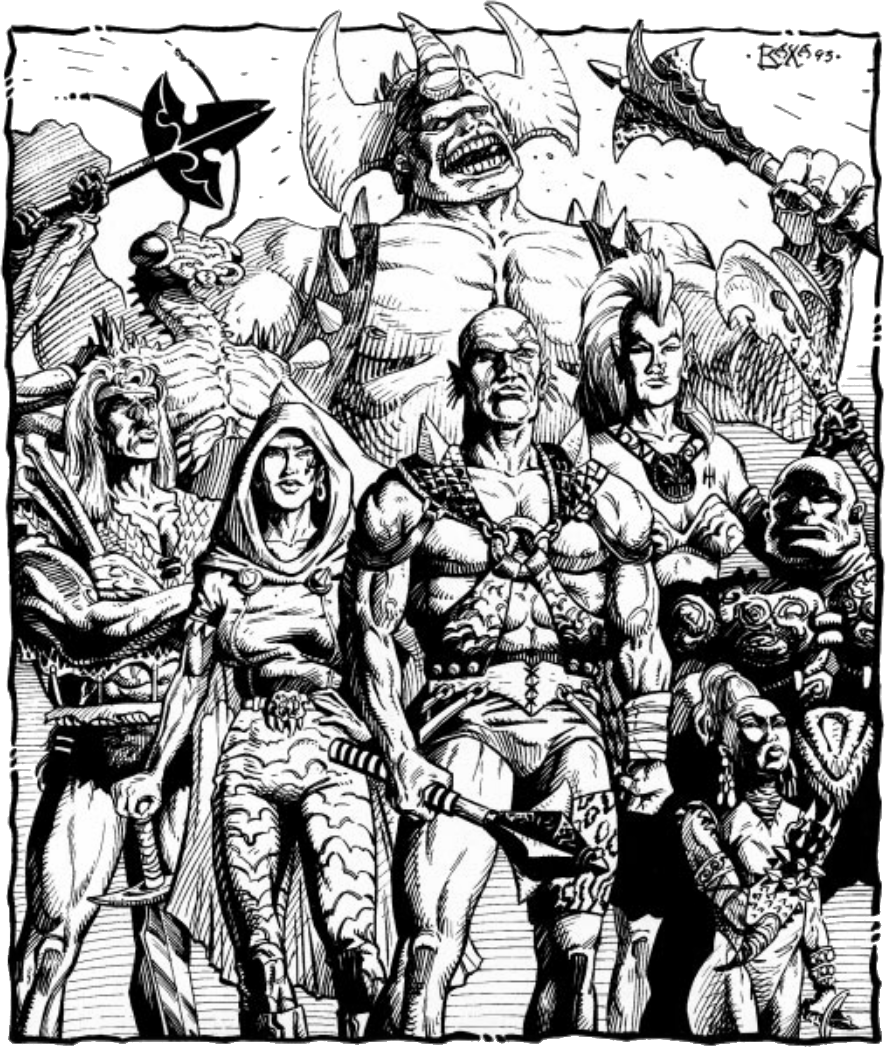
\includegraphics[width=\textwidth-22mm]{images/sizes-1.png}
\WOTC
\end{figure*}

\BigTablePair{Creature Size and Scale}{l*{3}{Z{12mm}}XX*{3}{Z{14mm}}}{
\tableheader Size Category &
\tableheader Size\footnotemark[1] Modifier &
\tableheader Grapple\footnotemark[2] Modifier &
\tableheader Hide\footnotemark[3] Modifier &
\tableheader Height or Length\footnotemark[4] &
\tableheader Weight\footnotemark[5] &
\tableheader Space\footnotemark[6] &
\tableheader Natural Reach\footnotemark[6] (Tall) &
\tableheader Natural Reach\footnotemark[6] (Long)\\

Fine       & +8   & $-16$ & +16   & 15 cm or less  & 60 g or less        & 15 cm & 0 m   & 0 m   \\
Diminutive & +4   & $-12$ & +12   & 15 cm--30 cm   & 60 g--0.5 kg        & 30 cm & 0 m   & 0 m   \\
Tiny       & +2   & $-8$  & +8    & 30 cm--60 cm   & 0.5 kg--4 kg        & 75 cm & 0 m   & 0 m   \\
Small      & +1   & $-4$  & +4    & 60 cm--1.2 m   & 4 kg--30 kg         & 1.5 m & 1.5 m & 1.5 m \\
Medium     & +0   & +0    & +0    & 1.2 m--2.4 m   & 30 kg--250 kg       & 1.5 m & 1.5 m & 1.5 m \\
Large      & $-1$ & +4    & $-4$  & 2.4 m--4.8 m   & 250 kg--1 tonne     & 3 m   & 3 m   & 1.5 m \\
Huge       & $-2$ & +8    & $-8$  & 4.8 m--9.6 m   & 1 tonne--8 tonnes   & 4.5 m & 4.5 m & 3 m   \\
Gargantuan & $-4$ & +12   & $-12$ & 9.6 m--19.2 m  & 8 tonnes--62 tonnes & 6 m   & 6 m   & 4.5 m \\
Colossal   & $-8$ & +16   & $-16$ & 19.2 m or more & 62 tonnes or more   & 9 m   & 9 m   & 6 m   \\

\BigTableNote{9}{1 A creature's size modifier is applied to it's attack bonus and Armor Class.}\\
\BigTableNote{9}{2 See the Grapple special attack.}\\
\BigTableNote{9}{3 See the \skill{Hide} skill.}\\
\BigTableNote{9}{4 Biped's height, quadruped's body length (nose to base of tail)}\\
\BigTableNote{9}{5 Assumes that the creature is roughly as dense as a regular animal. A creature made of stone will weigh considerably more. A gaseous creature will weigh much less.}\\
\BigTableNote{9}{6 These values are typical for creatures of the indicated size. Some exceptions exist.}\\
}

\subsection{Big and Little Creatures}
% \subsection{Big and Little Creatures In Combat}
Creatures smaller than Small or larger than Medium have special rules relating to position, reach, and weapon size.

\textbf{Tiny, Diminutive, and Fine Creatures:} Very small creatures take up less than 1 square of space. This means that more than one such creature can fit into a single square. A Tiny creature typically occupies a space only 75 centimeters across, so four can fit into a single square. Twenty-five Diminutive creatures or 100 Fine creatures can fit into a single square.

Creatures that take up less than 1 square of space typically have a natural reach of 0 meters, meaning they can't reach into adjacent squares. They must enter an opponent's square to attack in melee. This provokes an attack of opportunity from the opponent. You can attack into your own square if you need to, so you can attack such creatures normally.

Since they have no natural reach, they do not threaten the squares around them. You can move past them without provoking attacks of opportunity. They also can't flank an enemy.

\textbf{Large, Huge, Gargantuan, and Colossal Creatures:} Very large creatures take up more than 1 square. For instance, a half-giant takes up a space 3 meters on a side (2 squares wide).

Creatures that take up more than 1 square typically have a natural reach of 3 meters or more, meaning that they can reach targets even if they aren't in adjacent squares.

Unlike when someone uses a reach weapon, a creature with greater than normal natural reach (more than 1.5 meter) still threatens squares adjacent to it. A creature with greater than normal natural reach usually gets an attack of opportunity against you if you approach it, because you must enter and move within the range of its reach before you can attack it. (This attack of opportunity is not provoked if you take a 1.5-meter step.)

Large or larger creatures using reach weapons can strike up to double their natural reach but can't strike at their natural reach or less.